	In this module you will learn
	\begin{itemize}
		\item How to create a mindmap.
	\end{itemize}

\hfill \\



\Heading{Mind Map}

A mind map is a tool to visually outline and organize ideas. Typically a key idea is the centre of a mind map and associated ideas are added to create a diagram that shows the flow of ideas. 

\begin{example}

Let us focus on the question: ``What is the best recycling system for Toronto?''

Then we can think of many different definitions for what the word ``best'' means:

\begin{itemize}
	\item The system that gets the most participation from the population, which can be measured by the fraction of the Toronto households participating in recycling;
	\item The system that costs the least amount of money for the city. How can this be measured?
	\item The system that processes the most amount of recyclables.
\end{itemize}

In the figure below, we focus on the definition of ``best'', with these three possible definitions branching off to be further explored.

\def\MindMapOne{
	\fill[color=Green!70!white] (0,0) rectangle (4,1) node[pos=.5] {\color{black}``Best'' recycling centre};
	\fill[color=BurntOrange] (6,2.5) rectangle (8,1.5) node[pos=.5] {\color{black}\begin{minipage}{40pt}\raggedright Most participation\end{minipage}};
	\fill[color=Goldenrod] (6,0) rectangle (8,1) node[pos=.5] {\color{black}\begin{minipage}{45pt}\raggedright Least cost to the city\end{minipage}};
	\fill[color=red!70!white] (6,-2) rectangle (8,-0.5) node[pos=.5] {\color{black}\begin{minipage}{50pt}\raggedright Processes the most recyclables\end{minipage}};
	\draw (4,0.75) -- (6,2);
	\draw (4,0.5) -- (6,0.5);
	\draw (4,0.25) -- (6,-1.25);
%
%	\fill[color=Green!60!white] (0,0) rectangle (4,1) node[pos=.5] {\color{black}``Best'' recycling centre};
%	\fill[color=BurntOrange] (7,2.5) rectangle (11,1.5) node[pos=.5] {\color{black}Most participation};
%	\fill[color=Goldenrod] (7,0) rectangle (11,1) node[pos=.5] {\color{black}Least cost to the city};
%	\fill[color=red] (7,-1.5) rectangle (12,-0.5) node[pos=.5] {\color{black}Processes the most recyclables};
%	\draw (4,0.75) -- (7,2);
%	\draw (4,0.5) -- (7,0.5);
%	\draw (4,0.25) -- (7,-1);
}

\begin{center}
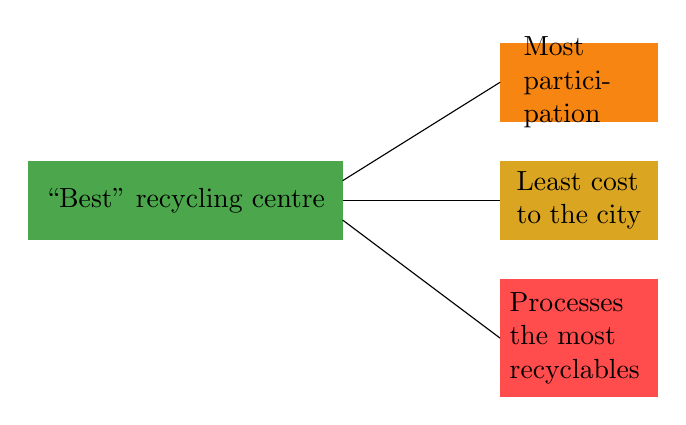
\begin{tikzpicture}
\MindMapOne
%	\fill[color=Green] (0,0) rectangle (4,1) node[pos=.5] {\color{black}``Best'' recycling centre};
%	\fill[color=BurntOrange] (7,2.5) rectangle (11,1.5) node[pos=.5] {\color{black}Most participation};
%	\fill[color=Goldenrod] (7,0) rectangle (11,1) node[pos=.5] {\color{black}Least cost to the city};
%	\fill[color=red] (7,-1.5) rectangle (12,-0.5) node[pos=.5] {\color{black}Processes the most recyclables};
%	\draw (4,0.75) -- (7,2);
%	\draw (4,0.5) -- (7,0.5);
%	\draw (4,0.25) -- (7,-1);
\end{tikzpicture}
\end{center}

 From here, we can focus our attention on one of the branches at a time.



%\end{example}
%
%%
%%\begin{figure}[!ht]
%%\begin{tikzpicture}
%%	\fill[color=Green] (0,0) rectangle (4,1) node[pos=.5] {\color{black}``Best'' recycling centre};
%%	\fill[color=BurntOrange] (7,2.5) rectangle (11,1.5) node[pos=.5] {\color{black}Most participation};
%%	\fill[color=Goldenrod] (7,0) rectangle (11,1) node[pos=.5] {\color{black}Least cost to the city};
%%	\fill[color=red] (7,-1.5) rectangle (12,-0.5) node[pos=.5] {\color{black}Processes the most recyclables};
%%	\draw (4,0.75) -- (7,2);
%%	\draw (4,0.5) -- (7,0.5);
%%	\draw (4,0.25) -- (7,-1);
%%\end{tikzpicture}
%%\caption{An example of a simple mind map.}
%%\label{mindmap1}
%%\end{figure}
%
%
%
%
%\begin{example}
%
Let's think about the least-cost option first. 

We probably can't determine how much any recycling program costs without knowing more about the recycling program, so a good place to start is to ask the question ``What kinds of recycling programs exist?''

If we aren't familiar with different types of recycling, we might need to do some research to see what kinds of programs exist.

A possible next step on your mind map for the least-cost approach could be expanding the mind map to the one shown below. %in the Figure \ref{mindmap2}.

\begin{center}
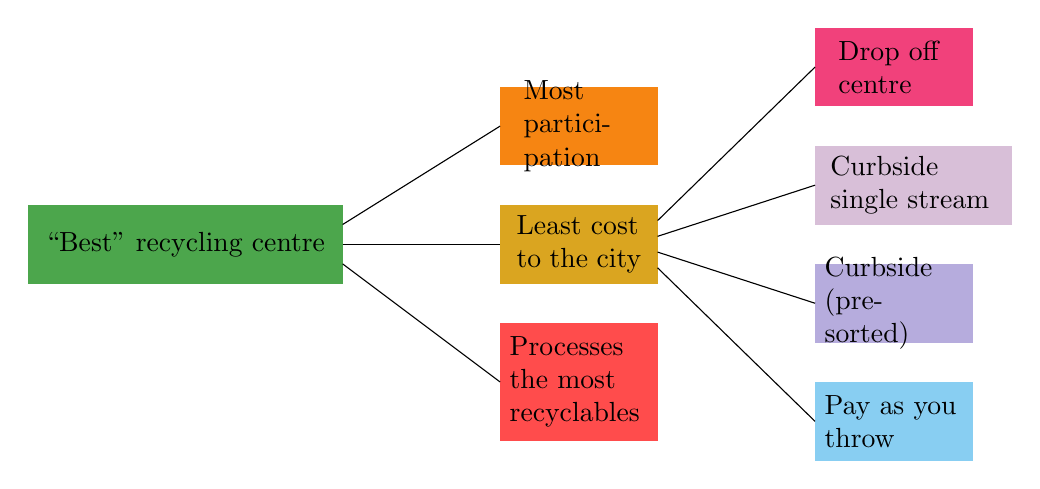
\begin{tikzpicture}
\MindMapOne
%	\fill[color=Green] (0,0) rectangle (4,1) node[pos=.5] {\color{black}``Best'' recycling centre};
%	\fill[color=BurntOrange] (6,2.5) rectangle (8,1.5) node[pos=.5] {\color{black}\begin{minipage}{40pt}\raggedright Most participation\end{minipage}};
%	\fill[color=Goldenrod] (6,0) rectangle (8,1) node[pos=.5] {\color{black}\begin{minipage}{45pt}\raggedright Least cost to the city\end{minipage}};
%	\fill[color=red] (6,-2) rectangle (8,-0.5) node[pos=.5] {\color{black}\begin{minipage}{50pt}\raggedright Processes the most recyclables\end{minipage}};
%	\draw (4,0.75) -- (6,2);
%	\draw (4,0.5) -- (6,0.5);
%	\draw (4,0.25) -- (6,-1.25);
	\fill[color=WildStrawberry!80!white] (10,2.25) rectangle (12,3.25) node[pos=.5] {\color{black}\begin{minipage}{40pt}\raggedright Drop off centre\end{minipage}};	
	\fill[color=Thistle] (10,0.75) rectangle (12.5,1.75) node[pos=.5] {\color{black}\begin{minipage}{60pt}\raggedright Curbside single stream\end{minipage}};	
	\fill[color=Periwinkle!50!white] (10,0.25) rectangle (12,-0.75) node[pos=.5] {\color{black}\begin{minipage}{50pt}\raggedright Curbside (pre-sorted)\end{minipage}};	
	\fill[color=Cerulean!50!white] (10,-2.25) rectangle (12,-1.25) node[pos=.5] {\color{black}\begin{minipage}{50pt}\raggedright Pay as you throw\end{minipage}};
	\draw (8,0.8) -- (10,2.75);	
	\draw (8,0.6) -- (10,1.25);	
	\draw (8,0.4) -- (10,-0.25);	
	\draw (8,0.2) -- (10,-1.75);	
\end{tikzpicture}
\end{center}

\end{example}

%
%\begin{figure}[!htbp]
%\begin{tikzpicture}
%	\fill[color=Green] (0,0) rectangle (4,1) node[pos=.5] {\color{black}``Best'' recycling centre};
%	\fill[color=BurntOrange] (6,2.5) rectangle (8,1.5) node[pos=.5] {\color{black}\begin{minipage}{40pt}\raggedright Most participation\end{minipage}};
%	\fill[color=Goldenrod] (6,0) rectangle (8,1) node[pos=.5] {\color{black}\begin{minipage}{45pt}\raggedright Least cost to the city\end{minipage}};
%	\fill[color=red] (6,-2) rectangle (8,-0.5) node[pos=.5] {\color{black}\begin{minipage}{50pt}\raggedright Processes the most recyclables\end{minipage}};
%	\draw (4,0.75) -- (6,2);
%	\draw (4,0.5) -- (6,0.5);
%	\draw (4,0.25) -- (6,-1.25);
%	\fill[color=WildStrawberry] (10,2.25) rectangle (12,3.25) node[pos=.5] {\color{black}\begin{minipage}{40pt}\raggedright Drop off centre\end{minipage}};	
%	\fill[color=Thistle] (10,0.75) rectangle (12.5,1.75) node[pos=.5] {\color{black}\begin{minipage}{60pt}\raggedright Curbside single stream\end{minipage}};	
%	\fill[color=Periwinkle] (10,0.25) rectangle (12,-0.75) node[pos=.5] {\color{black}\begin{minipage}{50pt}\raggedright Curbside (pre-sorted)\end{minipage}};	
%	\fill[color=Cerulean] (10,-2.25) rectangle (12,-1.25) node[pos=.5] {\color{black}\begin{minipage}{50pt}\raggedright Pay as you throw\end{minipage}};
%	\draw (8,0.8) -- (10,2.75);	
%	\draw (8,0.6) -- (10,1.25);	
%	\draw (8,0.4) -- (10,-0.25);	
%	\draw (8,0.2) -- (10,-1.75);	
%\end{tikzpicture}
%\caption{Next step of a mind map.}
%\label{mindmap2}
%\end{figure}


\begin{important}
		There is free online software to help creating a mind map. One such is \href{http://freemind.sourceforge.net}{FreeMind (http://freemind.sourceforge.net)}.
		
		\hfill \qrcode{http://freemind.sourceforge.net}		
\end{important}



